\documentclass[dvipsnames]{../../../../AritzhClass}

\usepackage{array}
\usepackage{arydshln}

\makeatletter
\renewcommand*\env@matrix[1][*\c@MaxMatrixCols c]{%
  \hskip -\arraycolsep
  \let\@ifnextchar\new@ifnextchar
  \array{#1}}
\makeatother

\usetikzlibrary{calc}
\lstset{
	language=C,
	showstringspaces=false,
	numbers=none,
	xleftmargin=0cm
}

\izenburua{Bonba}
\azpiizenburua{Proiektuaren Txostena}
\smalltitle{Bonba: Txostena}
\ikasgaia{Ingeniaritza Informatikoa: KE}
\author{Aritz Lopez}
\data{\today}

\begin{document}

\izenburuorrialdea

\tableofcontents

\pagebreak

\section{Proiektuaren enuntziatua}

Nintendo DS-rako \textit{100 doors} jokuaren motako ate bat diseinatu eta programatu, DS-aren pantaila, teklatua eta denboragailua erabiliz.

\section{Proiektuaren definizioa: Bonba}

Ebazpenerako pentsatu dugun atea zeran datza: Ukimen pantailan bonba bat agertuko da, 5 kablerekin, eta jokalariak kable egokia moztu behar izango du 10 segunduren barruan, bonba lehertu ez dadin. Jokoaren berjokagarritasuna honakoan datza: jokalariak kable desegokia pultsatuz gero, berriro saiatzeko aukera izango du (\textit{A} tekla pultsatuz gero); honela, aurreko kable bera pultsatu beharko du. Bestela, galtzean \textit{B} tekla pultsatzen badu, ausazko beste kable bat izango da moztu behar dena.

\section{Kontzeptu-mapa}

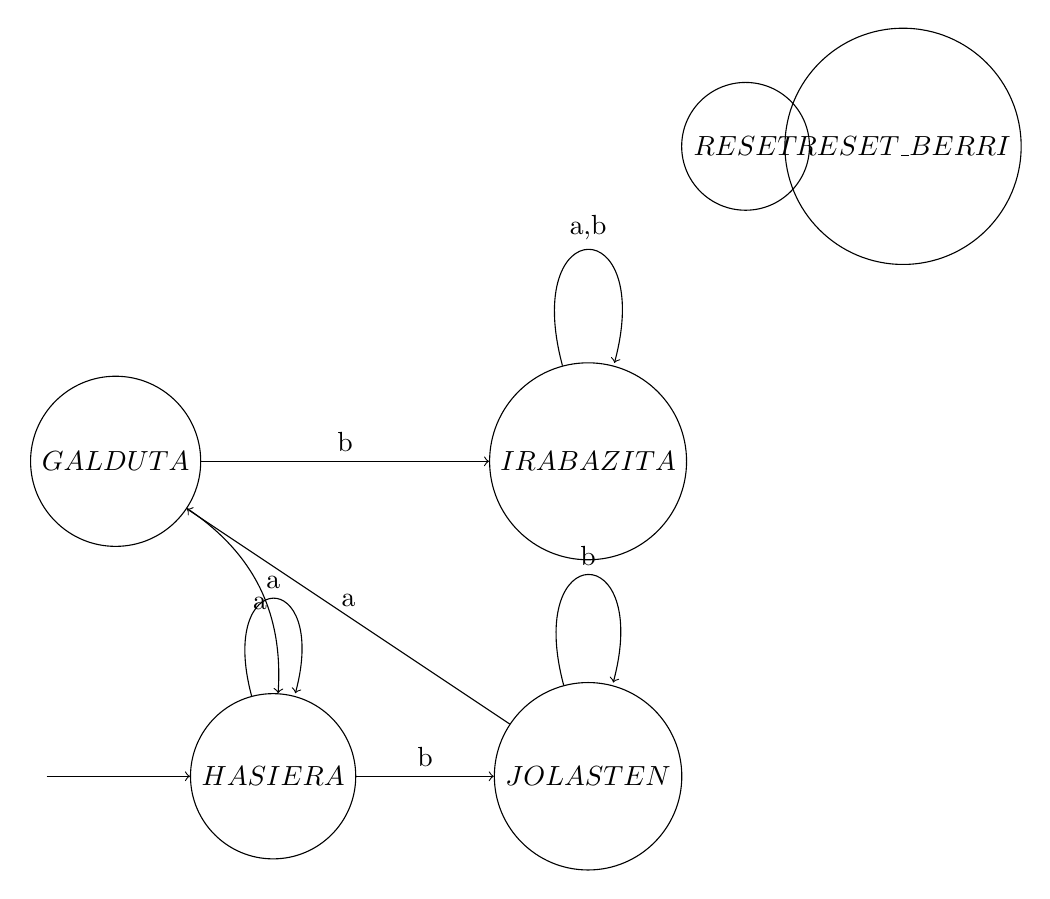
\begin{tikzpicture}
\node(pseudo) at (-1,0){};
\node(0) at (2,0)[shape=circle,draw]        {$HASIERA$};
\node(1) at (6,0)[shape=circle,draw]        {$JOLASTEN$};
\node(2) at (0,4)[shape=circle,draw]        {$GALDUTA$};
\node(3) at (6,4)[shape=circle,draw] {$IRABAZITA$};
\node(4) at (8,8)[shape=circle,draw] {$RESET$};
\node(5) at (10,8)[shape=circle,draw] {$RESET\_BERRI$};
\path [->]
  (0)      edge                 node [above]  {b}     (1)
  (1)      edge                 node [above]  {a}     (2)
  (2)      edge                 node [above]  {b}     (3)
  (2)      edge [bend left=30]  node [below]  {a}     (0)
  (0)      edge [loop above]    node [above]  {a}     ()
  (1)      edge [loop above]    node [above]  {b}     ()
  (3)      edge [loop above]    node [above]  {a,b}   ()
  (pseudo) edge                                       (0);
\end{tikzpicture}

\end{document}
